\documentclass[a6paper]{article}

\usepackage[total={8.9cm,13cm}, top=.8cm, left=.9cm, includefoot]{geometry}
\usepackage{graphicx}

\usepackage[czech]{babel}
\usepackage[utf8]{inputenc}

\usepackage {abstract}


\newcommand*\podpis{\hspace*{0em plus 1fill}\makebox{..........}}

\renewcommand{\abstractname}{ }

%\pagestyle{empty}
\begin{document}


\author {Anpetu}

\title{\textbf{Akičita čikalan}}
\date{}
\maketitle
\begin{center}
	
{\large
Malý bojovník
}



\vspace{60pt}
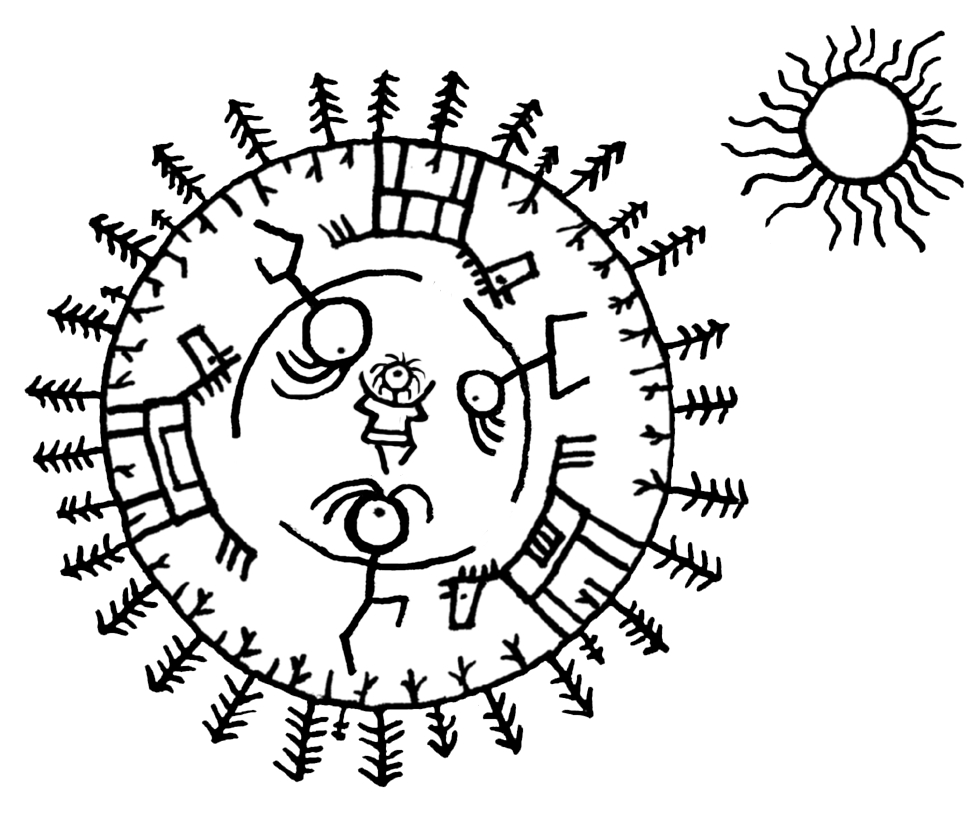
\includegraphics[width=0.6\textwidth]{piktogramy/agles_kluci_kruh.jpg}
\end{center}
\clearpage

\vspace*{15 pt}

\begin{Large}
{Bojovnice, bojovníci,}	
\end{Large}


\vspace{12 pt}
\begin{large}
	
vydali jste se s naším kmenem na dlouhou cestu. Tento sešítek vám bude radit, jaké dovednosti na ní využijete.


\vspace{25 pt}

S vašimi udi budete společně plnit úkoly. U každého splněného úkolu vám uďa podepíše políčko vpravo. 

\end{large}

\clearpage

\section*{Zdatnost} % (fold)
\label{sec:zdatnost}
\begin{itemize}
	\item Uběhnu 300 m členitým terénem \podpis
	\item Ušel jsem za jeden den aspoň 12 km \podpis
	\item Přeskočím svou délku (horizntálně) \podpis
\end{itemize}


% section zdatnost (end)


\section*{Oddíl a skauting} % (fold)
\label{sec:skauting}
\begin{itemize}
	\item Vím, kdo se zasloužil o vznik skautingu u nás \podpis
	\item Vím, jak vznikl náš oddíl \podpis
	\item Byl jsem aspoň na dvou oddílových akcích \podpis
	\item Znám telefonní číslo na své Uďi \podpis
	\item Znám oddílový pokřik \podpis
\end{itemize}
% section skauting (end)

\vspace{\fill}

\begin{center}
	
\includegraphics[width=0.3\textwidth]{piktogramy/indos_bezi2.jpg}
\end{center}
\clearpage


\section*{Uzly} % (fold)
\label{sec:uzly}
\begin{itemize}
	\item Umím si zavázat pohorky \podpis
	\item Uvážu lodní smyčku \podpis
\end{itemize}
% section uzly (end)


\section*{Tábornictví} % (fold)
\label{sec:tabornictvi}
\begin{itemize}
	\item S kamarádem dokážu uříznout polínko a rozštípnu ho  \podpis
	\item  Vím, co mám mít na družinovku a celý měsíc jsem nic nezapomněl  \podpis
	\item Umím si zabalit na vícedenní výpravu sám  \podpis

\end{itemize}
% section tábornictví (end)


\section*{Já a svět} % (fold)
\label{sec:ja_a_sv}
\begin{itemize}
	\item Zúčastním se dobročinné akce s oddílem.	 \podpis
	\item Vím, jak se dostat z klubovny domů.	 \podpis
\end{itemize}
% section ja_a_sv (end)


\begin{center}
	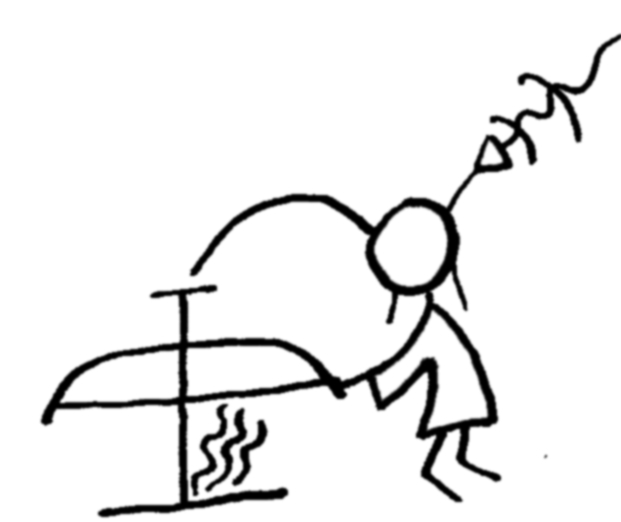
\includegraphics[width=0.35\textwidth]{piktogramy/agles_rozdelava_ohynek.jpg}
\end{center}
\clearpage


\section*{Zdravověda} % (fold)
\label{sec:zdrav}
\begin{itemize}
	\item Znám čísla IZS	 \podpis
	\item Vím, co dělat, když se spálím o kamna	 \podpis
	\item Umím ošetřit rozbité koleno	 \podpis
	\item Co udělám, když mě bodne vosa? 	 \podpis

\end{itemize}
% section zdrav (end)


\section*{Topografie} % (fold)
\label{sec:topografie}
\begin{itemize}
	\item Dokážu najít na mapě místo, kde se nacházím. \podpis
	\item Během jedné výprava si zkusím družinku vést. Nechám si ukázat, kudy půjdeme a potom trasu sleduji.		\podpis

\end{itemize}
% section topografie (end)
\vspace{\fill}
\begin{center}
	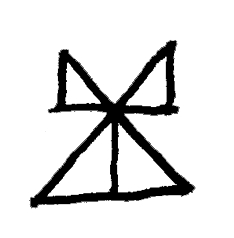
\includegraphics[width=0.25\textwidth]{piktogramy/typka.jpg}
\end{center}
%\vspace{10pt}
\clearpage

\section*{Tvořivost} % (fold)
\label{sec:tvorivost}
\begin{itemize}
	\item Uvařím čaj z přírodních surovin \podpis
	\item Vyberu si jeden z úkolů:
	\begin{itemize}
		\item vyřežu něco ze dřeva/kůry \podpis
		\item složím básničku nebo napíšu svou vlastní pohádku (aspoň 15 vět) \podpis
		\item upletu si náramek \podpis
		\item naučím se 3 akordy na kytaru/ukulele \podpis
	\end{itemize}

\end{itemize}
% section tvorivost (end)



\section*{Šifry} % (fold)
\label{sec:sifry}
\begin{itemize}
	\item Naučím se šifru zvanou mřížka. Dokážu rozluštit zprávu a napsat tři věty.\podpis
	\item S nápovědou rozluštím zprávu v morseovce, dokážu se morseovkou podepsat.\podpis
\end{itemize}
% section sifry (end)
\vspace{\fill}
\begin{center}
	
\includegraphics[width=0.7\textwidth]{piktogramy/korale.jpg}
\end{center}
\clearpage


\section*{Příroda} % (fold)
\label{sec:priroda}
\begin{itemize}
	\item Znám 5 jehličnatých a 5 listnatých stromů, vím, jak vypadají a dokážu je určit v přírodě.\podpis
\item Vyberu si divoké zvíře žijící v ČR, zjistím si o něm informace a povím o něm ostatním.\podpis
\item Vyberu si jeden z úkolů:
\begin{itemize}
	\item Naučím se poznat 5 stop lesní zvěře. \podpis
	\item Naučím se poznat  5 divoce rostoucích bylin a vím, na co která pomáhá. \podpis
	\item Naučím se rozeznat 5 ptáků podle zpěvu.\podpis

\end{itemize}

\end{itemize}
% section příroda (end)
\vspace{\fill}
\begin{center}
	
\includegraphics[width=0.5\textwidth]{piktogramy/mysicky.jpg}
\end{center}
\clearpage

\vspace*{50pt}
\begin{center}
	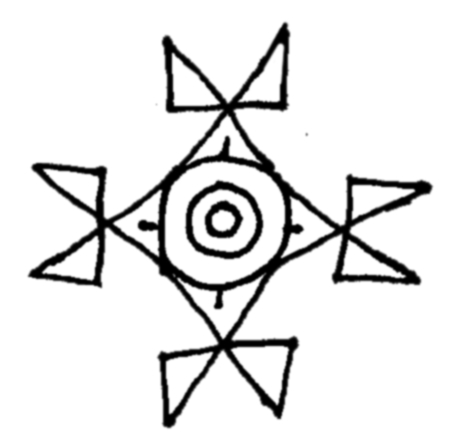
\includegraphics[width=0.5\textwidth]{piktogramy/symbol_kruh_4_typka.jpg}
\end{center}

\vspace{\fill}

\begin{tiny}
	\hspace{\fill}
	Stezky anpetu, V 1.0RC1
\end{tiny}

\end{document}